\documentclass[journal, onecolumn]{IEEEtran}
\IEEEoverridecommandlockouts


% En caso de requerir agregar algún paquete, favor de ponerlo en el archivo
% "paquetes.tex". Ahí ya están algunos, los más comunes para importar imágenes, 
% ecuaciones, símbolos e importar código. Según yo son los necesarios para hacer
% el reporte. Pero de igual forma verificar y agregar según conveniencia. 
\usepackage[spanish]{babel}
\usepackage[utf8]{inputenc}
\usepackage{cite}
\usepackage{amsmath,amssymb,amsfonts}
\usepackage{algorithmic}
\usepackage{graphicx}
\usepackage{textcomp}
\usepackage{xcolor}
\usepackage{fancyhdr}
\usepackage{listings}
\usepackage{float}
\usepackage{blindtext}
\usepackage{newtxmath}
\usepackage{wrapfig}
\usepackage{mathtools}
\usepackage{breqn}
\usepackage{titlesec}
\usepackage{multirow}

\usepackage[flushleft]{threeparttable}
\usepackage{makecell,booktabs}

\usepackage[hyphens]{url}
\usepackage[hidelinks]{hyperref}


\lstdefinestyle{code}{%
backgroundcolor=\color{gray!1},
basicstyle=\ttfamily\small,
commentstyle=\color{green!60!black},
keywordstyle=\color{magenta},
stringstyle=\color{blue!50!red},
showstringspaces=false,
%captionpos=b,
numbers=left,
numberstyle=\footnotesize\color{gray},
numbersep=5pt,
%stepnumber=2,
tabsize=2,
%frame=L,
%framerule=1pt,
%rulecolor=\color{red},
breaklines=true,
}

\hypersetup{breaklinks=true}


\titlespacing*{\section}
{0pt}{2.0ex plus 1ex minus .2ex}{1.0ex plus .2ex}
\titlespacing*{\subsection}
{0pt}{2.0ex plus 1ex minus .2ex}{1.0ex plus .2ex}
\titlespacing*{\subsubsection}
{0pt}{2.0ex plus 1ex minus .2ex}{1.0ex plus .2ex}

\renewcommand\IEEEkeywordsname{Palabras Clave}


\def\BibTeX{{\rm B\kern-.05em{\sc i\kern-.025em b}\kern-.08em
    T\kern-.1667em\lower.7ex\hbox{E}\kern-.125emX}}


\graphicspath{ {../Imagenes/} }

\numberwithin{equation}{section}
\numberwithin{figure}{section}
\numberwithin{table}{section}

\newcommand{\scaleFigures}{0.5}

\begin{document}
    \bstctlcite{IEEEexample:BSTcontrol}
    \title{Súper Resolución\\
    \small{Comparativa de técnicas}}

    
    \author{\IEEEauthorblockN{Madrigal-Custodio, Jesús A., Tevera-Ruiz Alejandro, Torres-Martínez Luis Á.\\}
    \IEEEauthorblockA{\textit{Departamento: Robótica y Manufactura Avanzada} \\
    \textit{Centro de Investigación y de Estudios Avanzados del Instituto Politécnico Nacional}}
    }

    \maketitle

    \begin{abstract}
        En el presente documento se explican los fundamentos, metodología y proceso de implementación 
        para el desarrollo de algoritmos de súper resolución bajo diversos enfoques con el objetivo... 
    \end{abstract}

    \begin{IEEEkeywords}
    Súper Resolución, Redes Convolucionales, Inteligencia Artificial
    \end{IEEEkeywords}

    \section{Introducción}
    % Comando para importar archivos en la plantilla.
    % Para ello deberá crear el archivo .tex en la carpeta "Secciones" 
    % Y posteriormente importarlo con el comando "input".

    % Cada que realice un cambio en el main favor de actualizarlo en el 
    % repo para no tener problemas en el manejo de este archivo que todos
    % moveremos. Lo mismo para el archivo paquetes.
    
    % Para el resto no es necesario. 


    
El gran reto de estimar una imagen de alta resolución, teniendo de base una imagen de baja calidad es a lo que se le conoce como 
\emph{Super Resolución},la Super-Resolución para una sola imagen (SISR) es un problema que ha sido estudiado desde antes del siglo XXI, lo que comenzó tiempo atrás
como un tema de ciencia ficción termino por ser un tema de investigación que aun no culmina, pero presenta avances significativos en la actualidad.
Existen muchos antecedentes sobre modelos que tratan de recuperar la información de las imágenes de baja resolución haciendo un escalado de esta y 
 con el uso de modelos probabilísticos estimar los datos faltantes, otros que aplican parches en combinación con imágenes de alta resolución para lograr un 
 resultado legible sentando un precedente en la investigación.
 
 A pesar de estos esfuerzos aun se buscaba mejorar estas estimaciones, con el surgimiento de las \emph{Redes Neuronales Artificiales}, capaces de realizar predicciones dada sus
habilidad de aprendizajes, podían obtener modelos precisos de una tarea especifica a partir de fragmentos de información con los cuales realizan un entrenamiento. De
esta nueva estrategia surgen entonces diferentes modelos de redes Neuronales como los son las Convolucionales, GAN´s, Residuales, entre otras.Esto 
se puede considerar hasta ahora el mayor avance en cuanto a super resolución.

El objetivo de este trabajo es realizar una comparativa entre 3 diferentes métodos para la obtención de Super Resolución, se consideran el algoritmo de Freeman \cite{freeman},
la Super resolución por Redes Neuronales Convolucionales \cite{SRCNN} y las Redes Generativas Adversarias \cite{SRGAN}. Al aplicar estos modelos se busca
visualizar claramente como se estructura cada uno, cuales son las ventajas y desventajas, cuantificar el avance tecnológico y dar un panorama sobre lo alcanzado en la actualidad
mediante la comparativa de resultados. 
    

    \section{Antecedentes}
    \begin{frame}{Súper Resolución}
    Bajo un enfoque \emph{clásico}, existen tres formas de mejorar la resolución 
    de una imagen:


    \begin{block}{Métodos}
        \begin{itemize}
            \item Amplificación de detalles existentes
            \item Suma de múltiples frames
            \item Único frame
        \end{itemize}
    \end{block}

\end{frame}

\begin{frame}{Predicción de resolución a partir de un único frame}
    ¿Cómo aumentar la densidad de pixeles de una imagen? 

    \pause
    \vspace{0.5cm}
    
    Predicción, aproximación... 
    
    \pause 

    \vspace{0.5cm}

    \begin{block}{Tipos}
        Dentro de las propuestas se encuentran los interpoladores:
        \begin{itemize}
            \item \emph{Adaptativos}: Algoritmos cambiantes por pixel
            \item \emph{No adaptativos}: Algoritmos estáticos a través de Algoritmos
            adyacentes. 
        \end{itemize}
    \end{block}

    Algunos de ellos incluyen algoritmos como \emph{vecino más cercano, bilineal, bicúbica,
    spline, entre otros.}
    
\end{frame}

\begin{frame}{Interpoladores no adaptativos}
    
    \begin{block}{Tipos}
        \begin{itemize}
            \item \textbf{Vecino más cercano} - Vecindad 1x1
            \item \textbf{Bilineal} - Vecindad 2x2 con promedios ponderados
            \item \textbf{Bicúbica} - Vecindad 4x4 con promedios ponderados 
        \end{itemize}
    \end{block}


    
    \begin{figure}[H]
        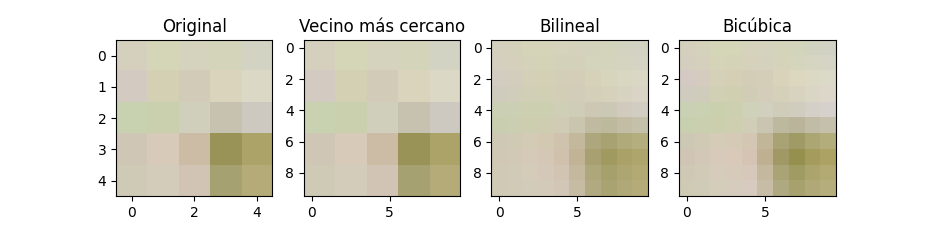
\includegraphics[scale = 0.45 ]{ tipos_interpoladores.png }
        \centering
        \caption{ Algoritmos de interpolación no adaptativos }
        \label{fig:interpoladores}
    \end{figure}

\end{frame}

\begin{frame}{Efectos de la interpolación}
    
    Todos los interpoladores no adaptativos intentan encontrar un equilibrio óptimo
    entre tres efectos no deseados: halos de borde, desenfoque y \emph{aliasing}. En la 
    Figura \ref{fig:efectos_inter} puede observarse el efecto para cada caso. 
    
    \begin{figure}[H]
        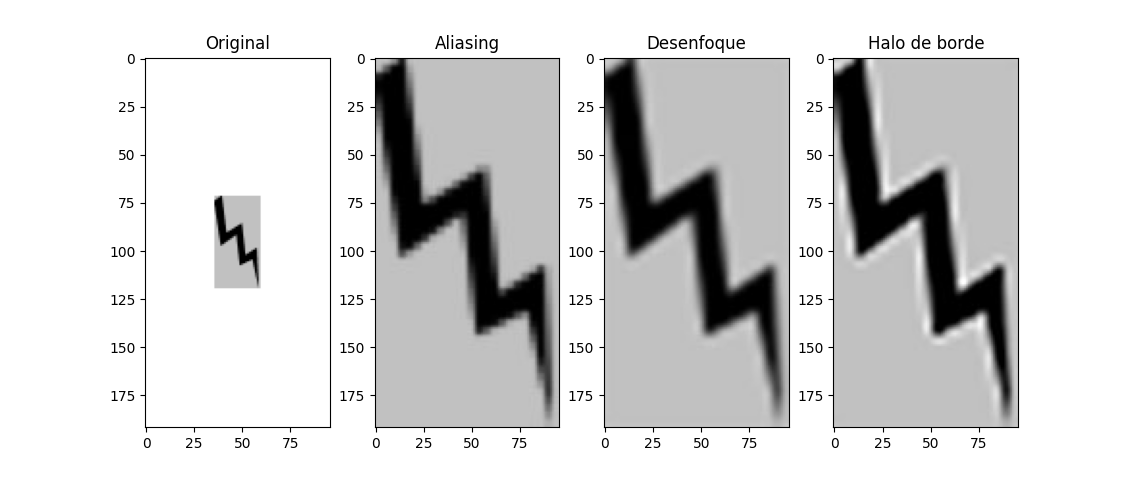
\includegraphics[scale = 0.35 ]{ efectos_inter.png }
        \centering
        \caption{ Efectos de interpolación}
        \label{fig:efectos_inter}
    \end{figure}

\end{frame}


\begin{frame}{Mejorar la interpolación de imágenes}
    
    \begin{block}{Dentro de las propuestas, \emph{Freeman et al} propone:}
        \begin{enumerate}
            \item La relación entre parches de alta y baja resolución
            es independiente del contraste de la imagen. 
            \item Los detalles están en las altas frecuencias 
        \end{enumerate}
    \end{block}

    \begin{figure}[H]
        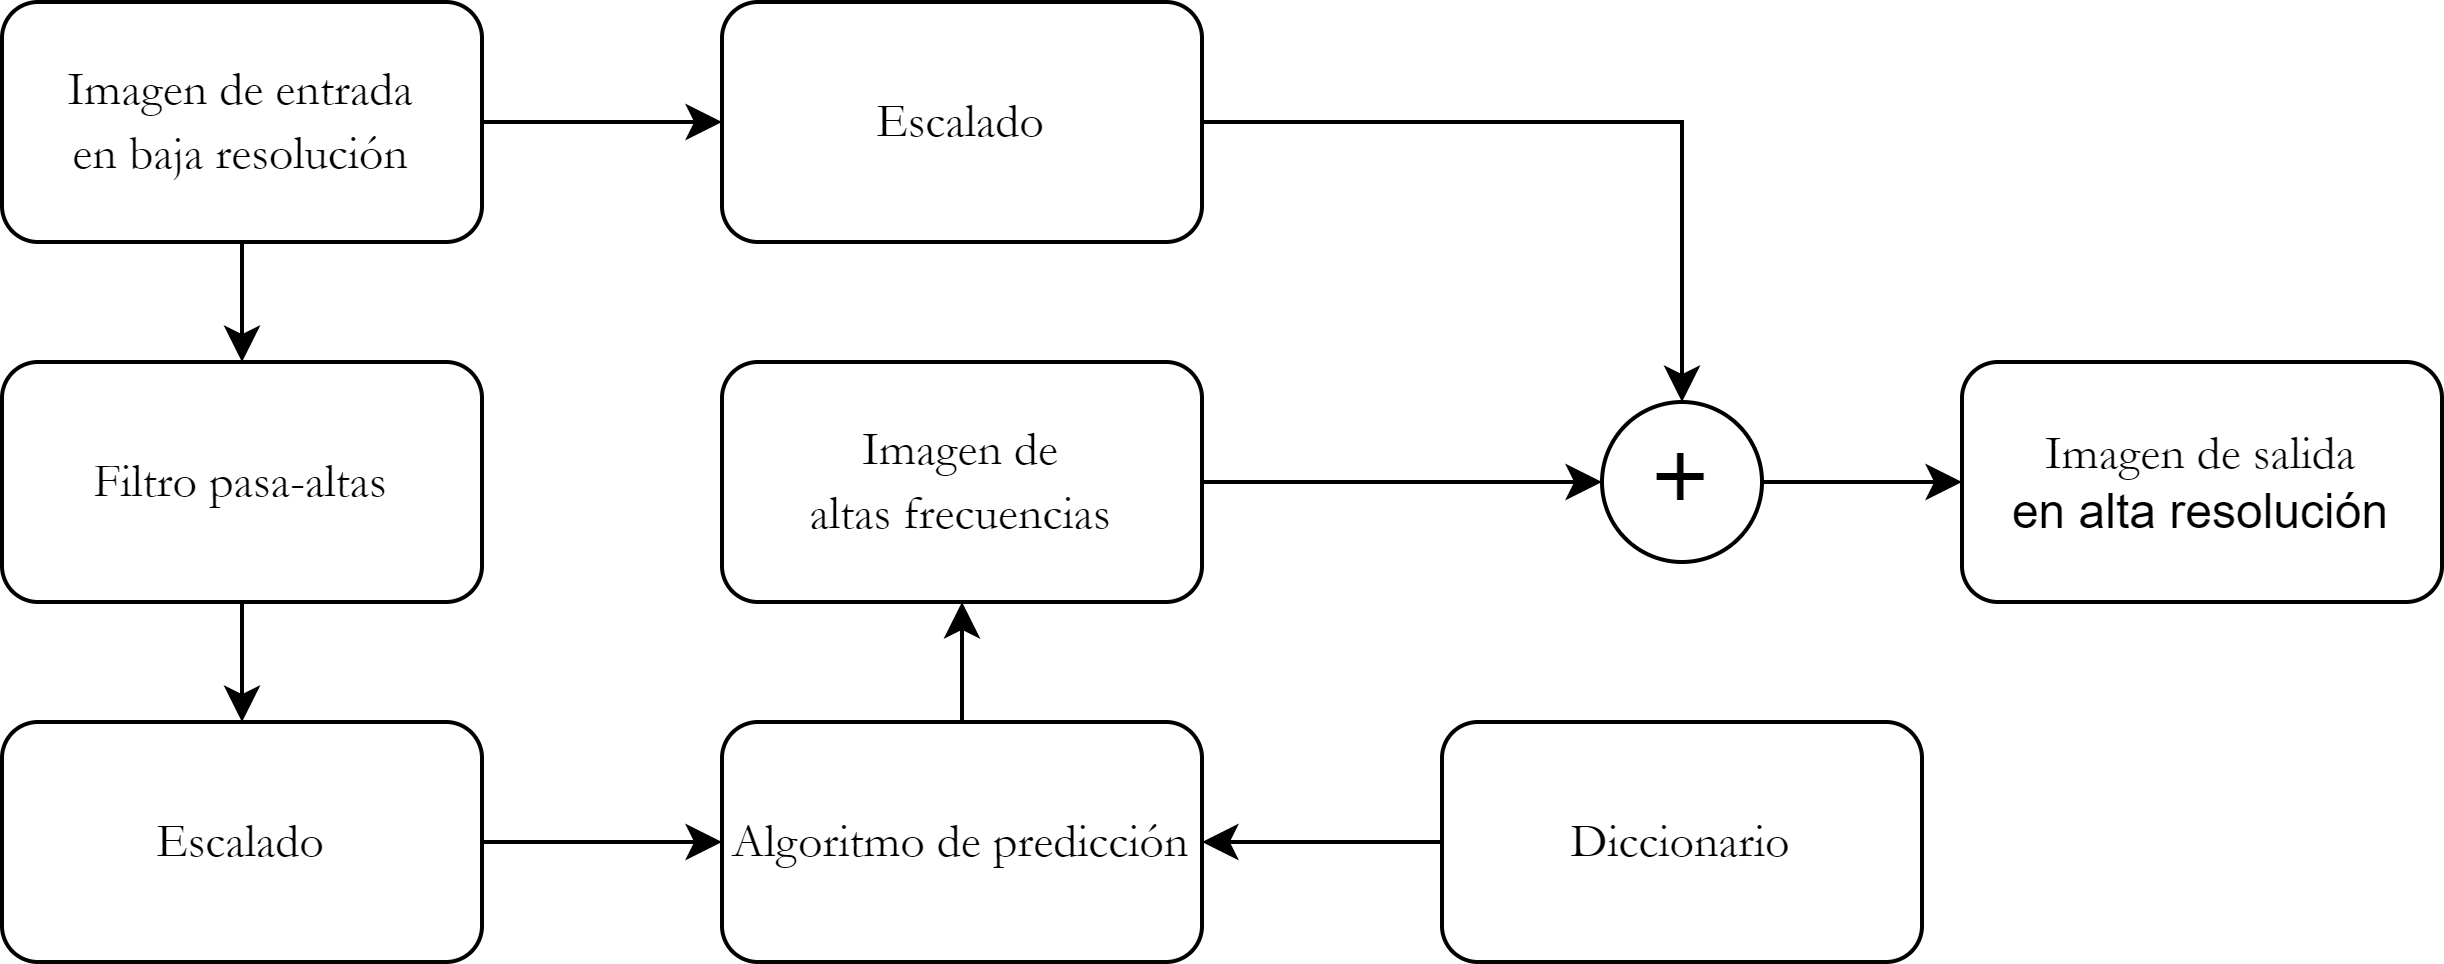
\includegraphics[scale = 0.4]{ fr_algoritmo.png }
        \centering
        \caption{ Algoritmo de súper resolución }
        \label{fig:fr_algoritmo}
    \end{figure}
    
\end{frame}

\begin{frame}{Diccionario}

    \begin{figure}[H]
        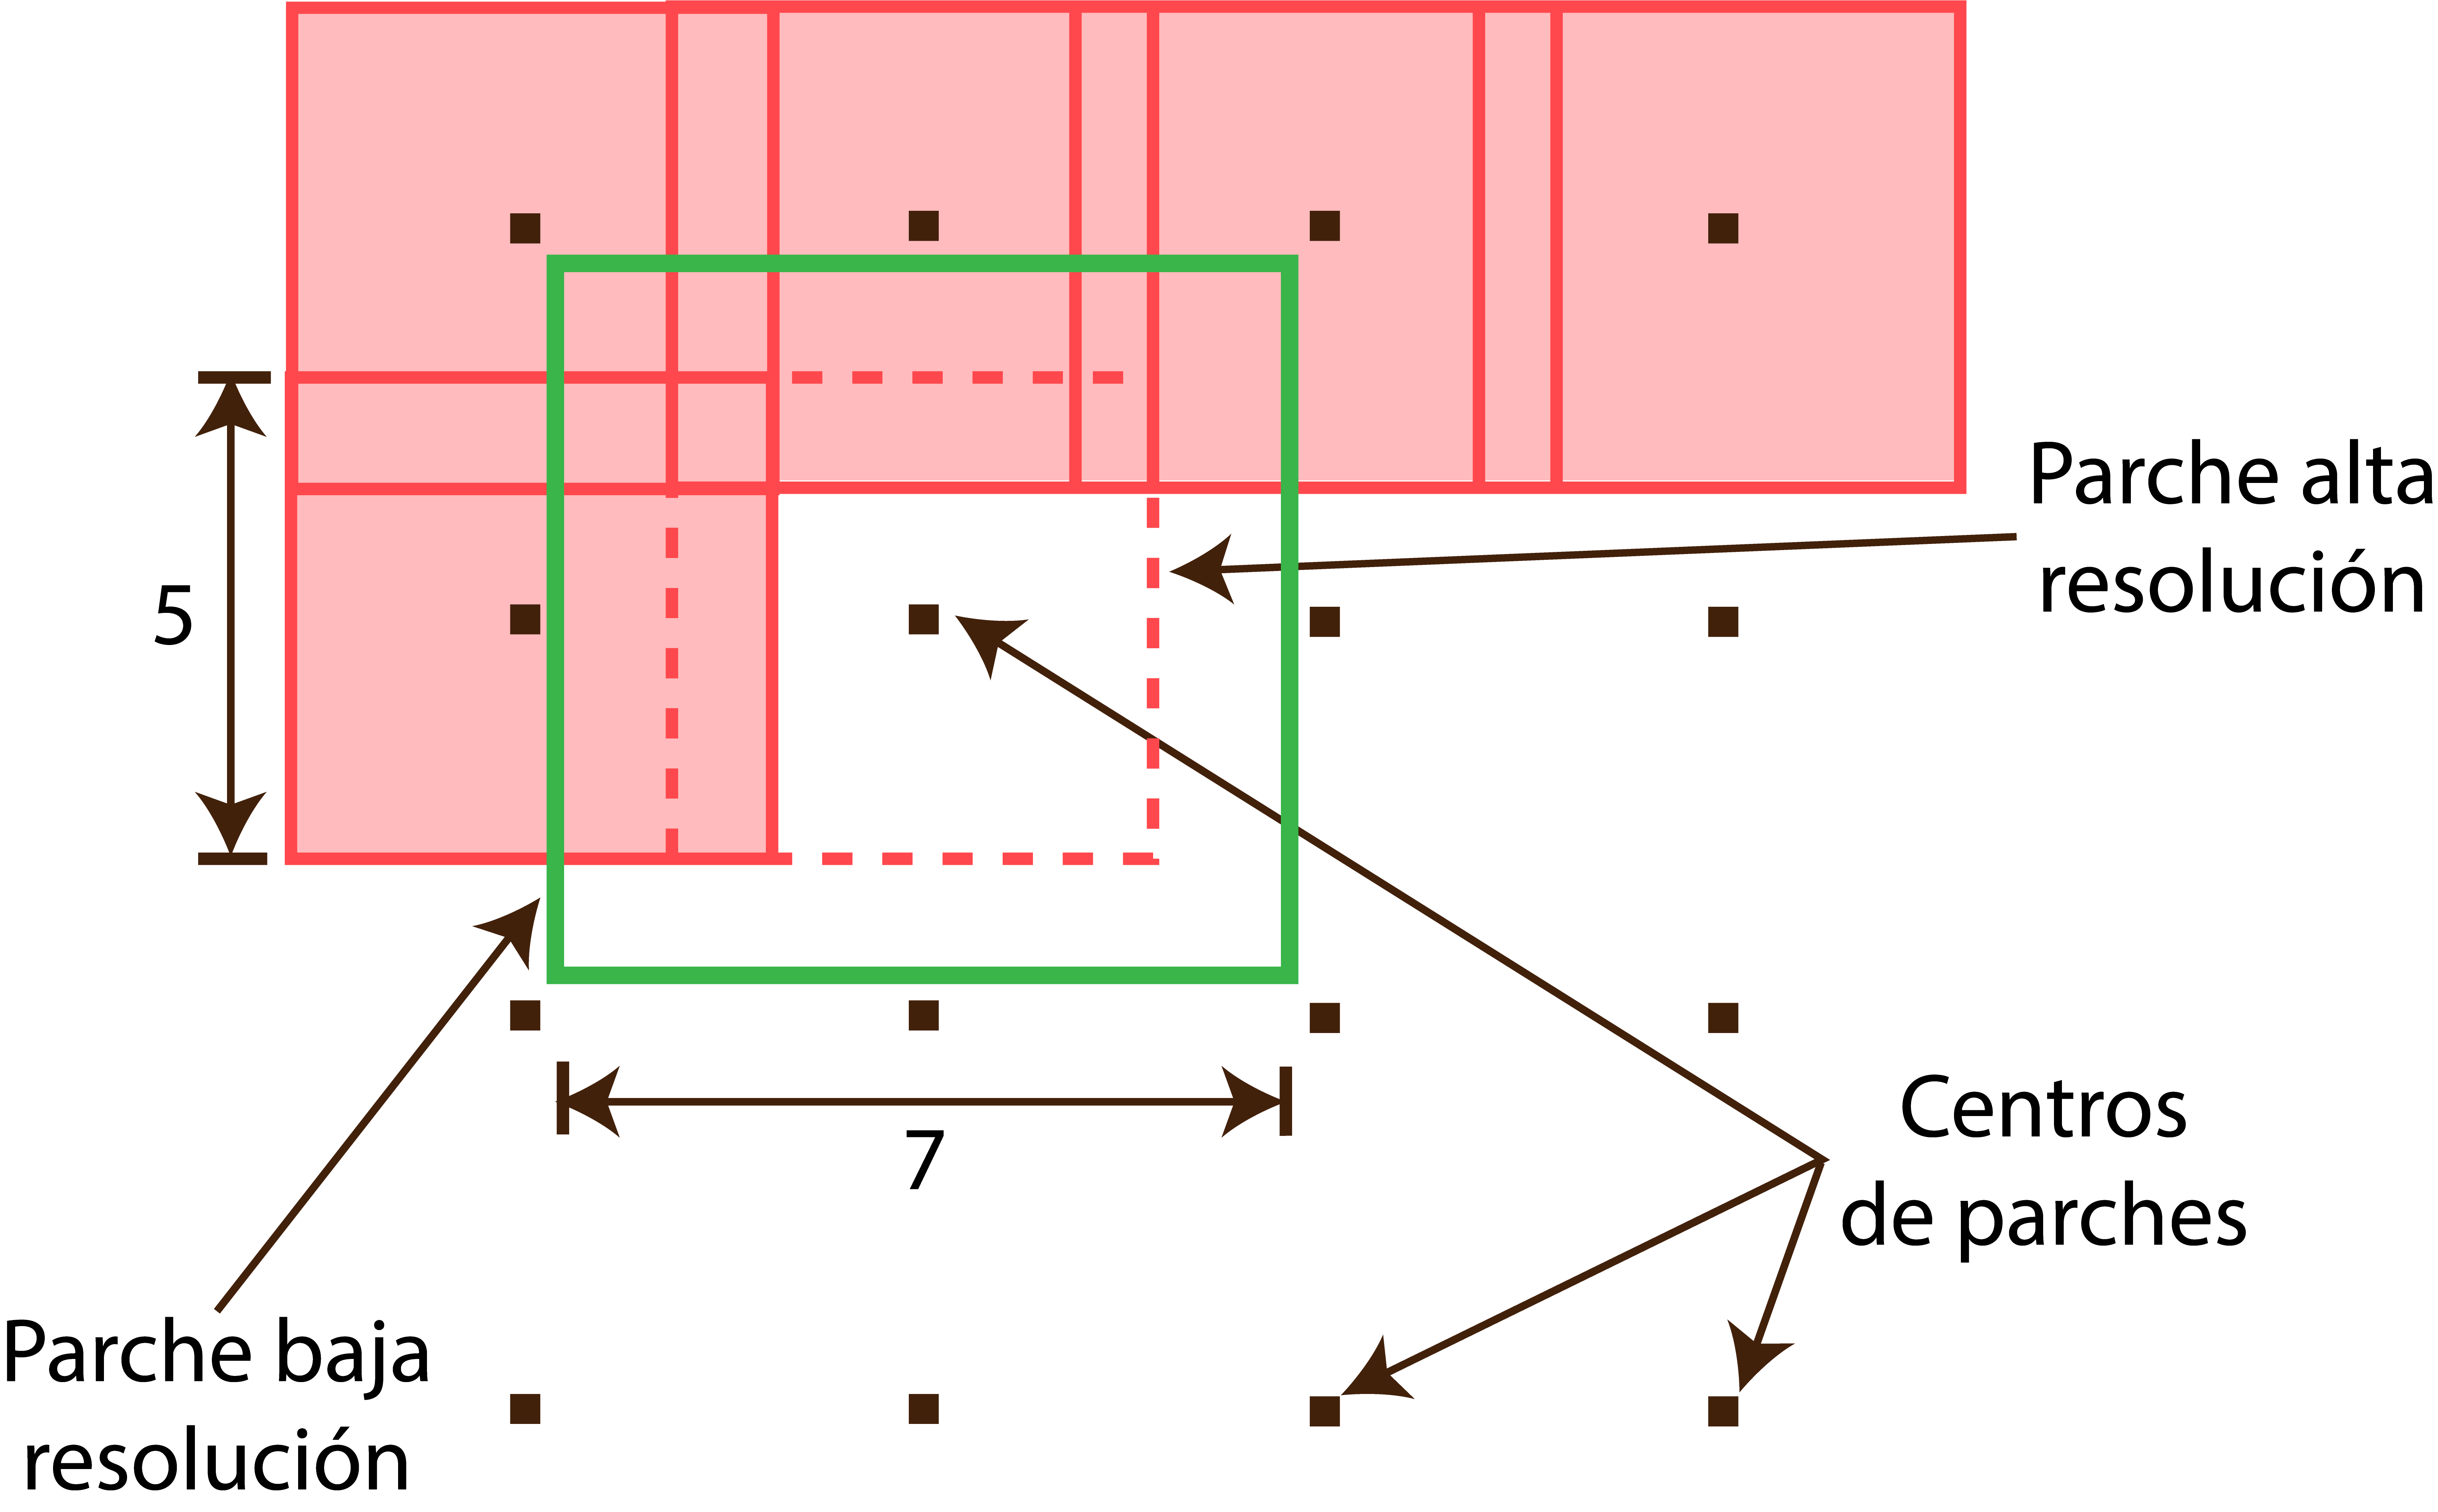
\includegraphics[scale = 0.18]{ fr_diccionario.png }
        \centering
        \caption{ Adquisición de parches de cada imagen}
        \label{fig:fr_dic}
    \end{figure}

    En específico, los parches de baja resolución deben reordenarse como un vector 
    en $\mathbb{R}^{1\times49}$ concatenado con la primera fila y primera columna
    del parche de alta resolución, resultando en un \textbf{vector para búsqueda} en $\mathbb{R}^{1\times59}$.
    
\end{frame}


\begin{frame}{Algoritmo de predicción}

    \begin{figure}[H]
        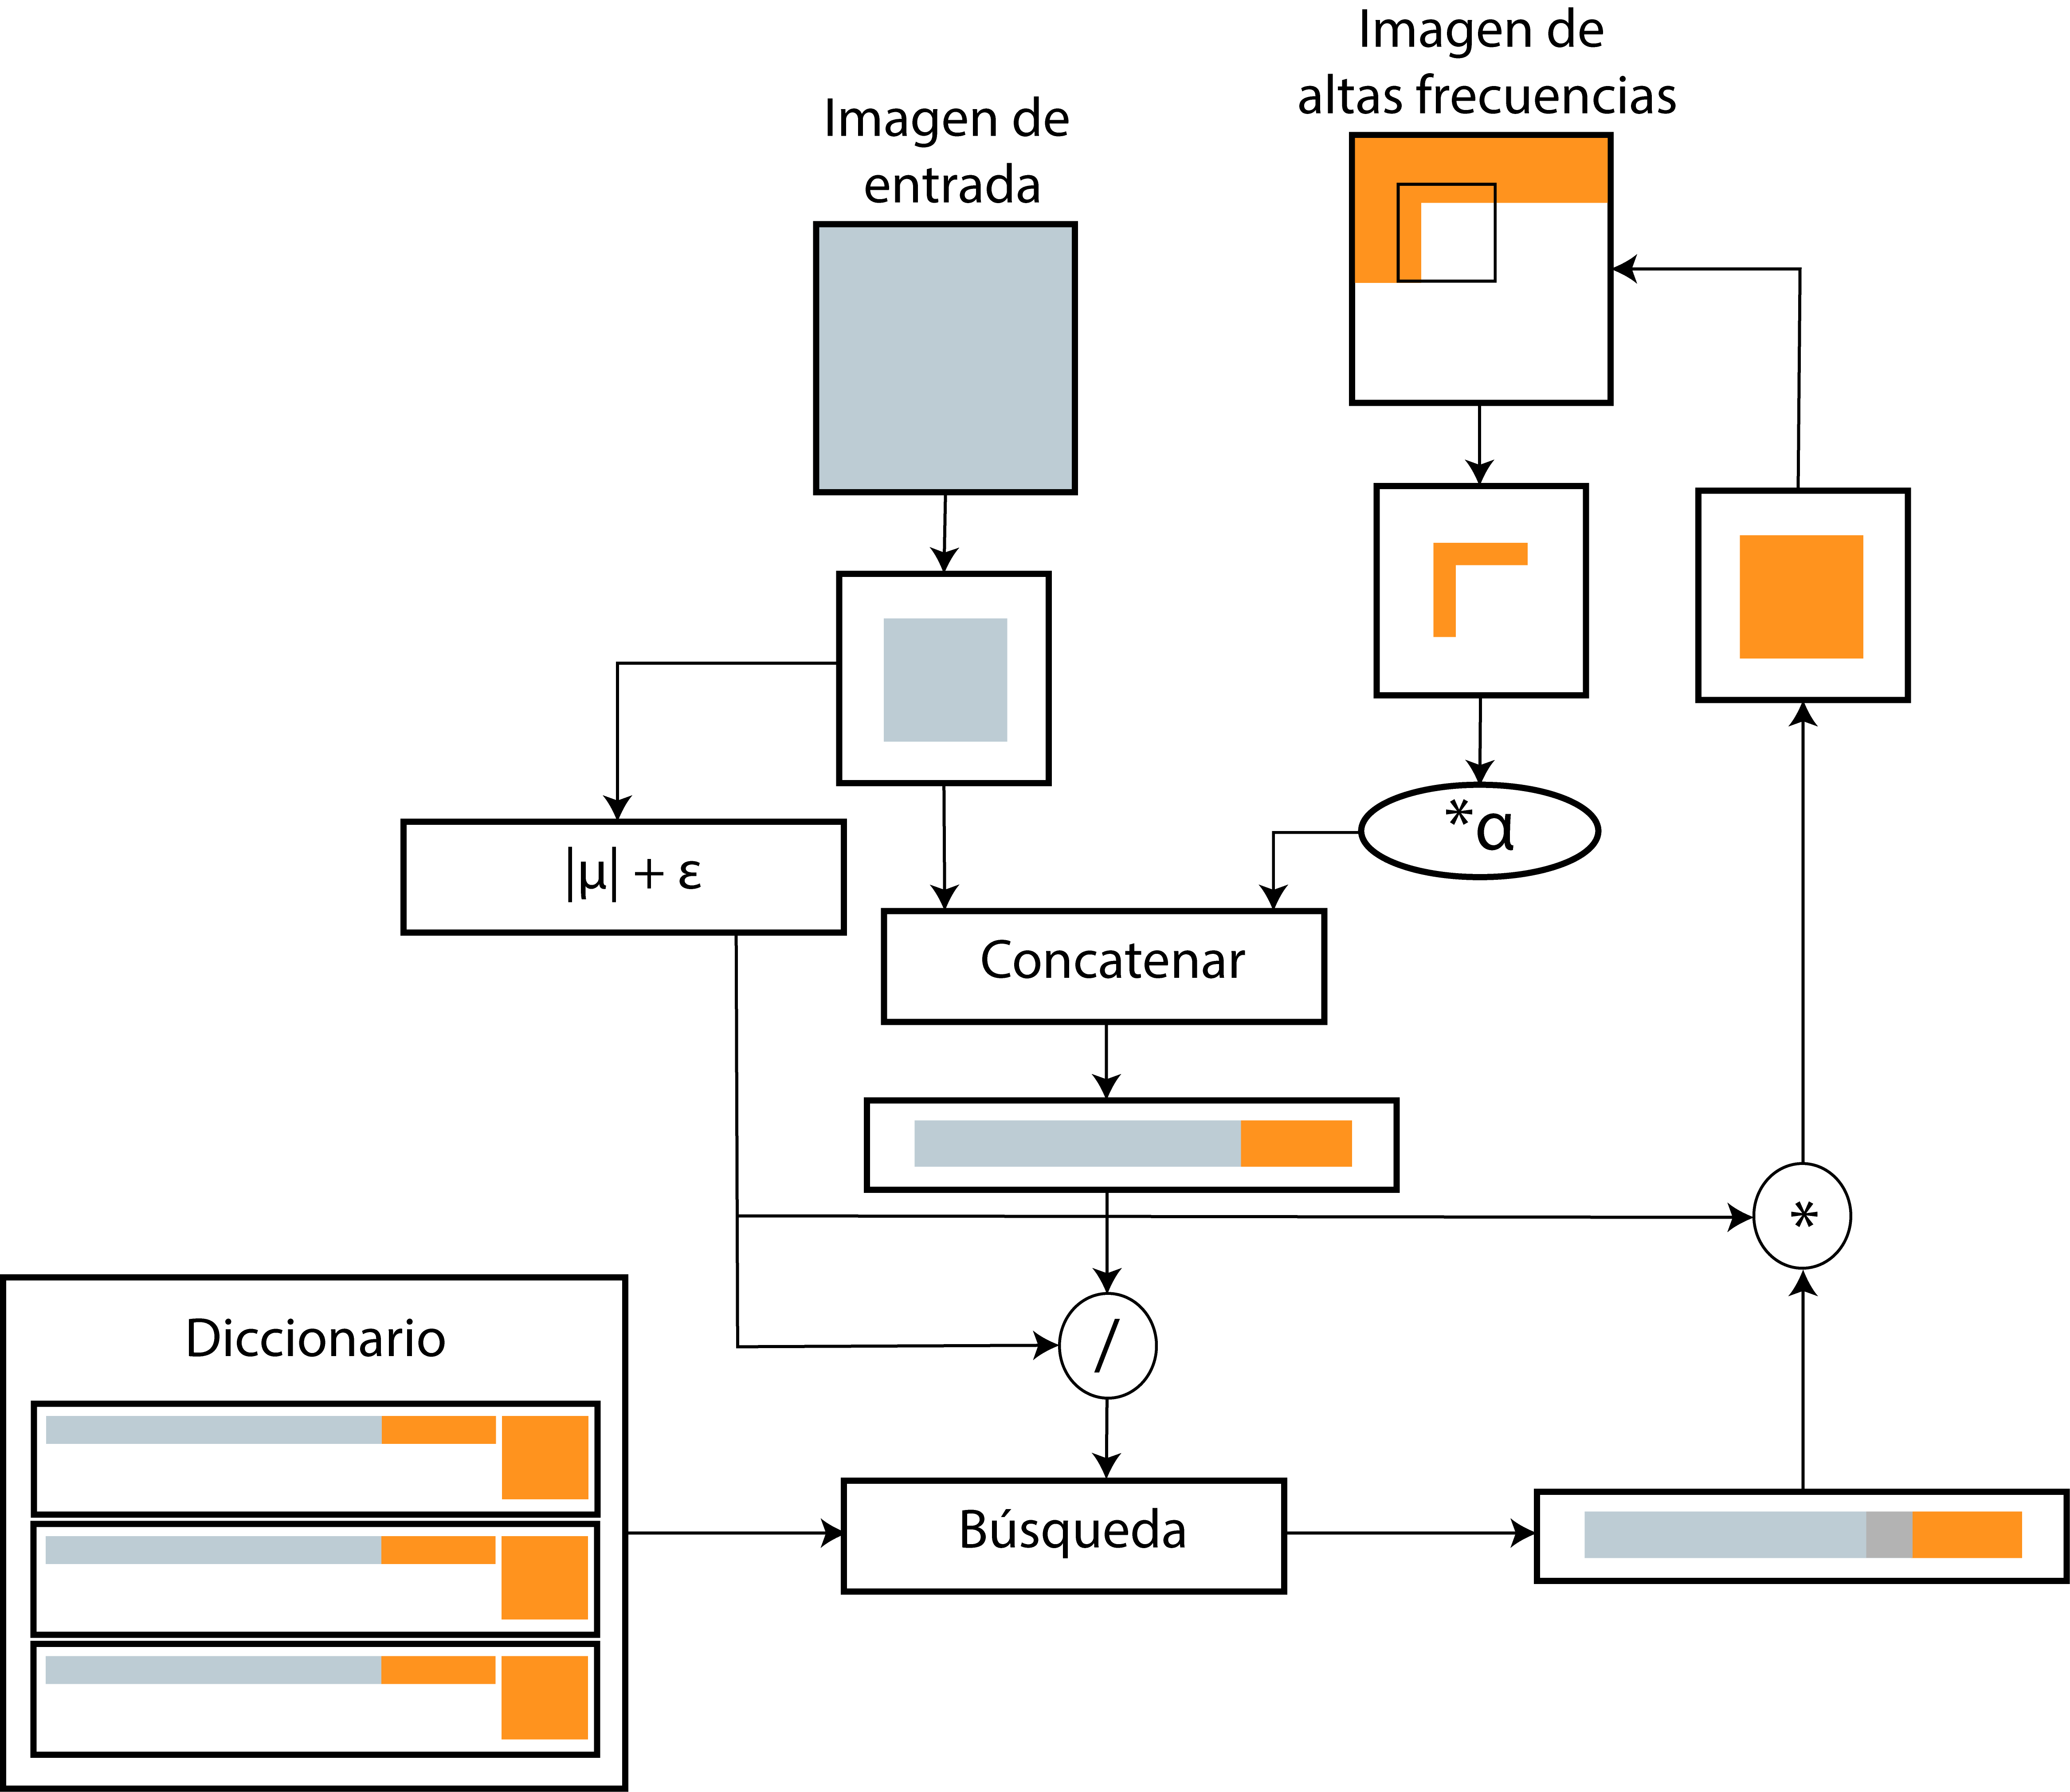
\includegraphics[scale = 0.3]{ freeman_prediccion.png}
        \centering
        \caption{ Algoritmo de predicción de imagen de frecuencias altas }
        \label{fig:fr_prediccion}
    \end{figure}

\end{frame}




    \section{Implementación}

    \section{Resultados}

    \section{Discusión}


    \section{Conclusiones}
    \noindent buenas buenas 


    \nocite{*}

    \Urlmuskip=0mu plus 1mu\relax
    \bibliographystyle{IEEEtran}
    \bibliography{bibliografia}

\end{document}